% This LaTeX was auto-generated from MATLAB code.
% To make changes, update the MATLAB code and export to LaTeX again.

\documentclass{article}

\usepackage[utf8]{inputenc}
\usepackage[T1]{fontenc}
\usepackage{lmodern}
\usepackage{graphicx}
\usepackage{color}
\usepackage{listings}
\usepackage{hyperref}
\usepackage{amsmath}
\usepackage{amsfonts}
\usepackage{epstopdf}
\usepackage{matlab}

\sloppy
\epstopdfsetup{outdir=./}
\graphicspath{ {./draft1_images/} }

\begin{document}

\matlabtitle{RX Basic Implementation}

\matlabheading{Introduction}

\begin{par}
\begin{flushleft}
THis notebook is meant to help implement the RX (and later the SSRX) algorithm on the RIT Blind Test data set.
\end{flushleft}
\end{par}

\begin{par}
\begin{flushleft}
The RX algorithm is given by: $\textrm{RX}={\left(\overrightarrow{X} -\overrightarrow{m} \right)}^T \phi^{-1} \left(\overrightarrow{X} -\overrightarrow{m} \right)>\mathrm{Threshold}$
\end{flushleft}
\end{par}

\begin{matlabcode}
file = 'G:\My Drive\Project\self_test\HyMap\self_test_rad.img';
[mat,hdr] = auto_load_HS(file);
\end{matlabcode}
\begin{matlaboutput}
Loading ENVI header ...
Loading ENVI image ...
\end{matlaboutput}
\begin{matlabcode}
data=double(permute(mat,[2,1,3]));
[x_size,y_size, num_of_bands]=size(data);
[X_MINUS_M,phi]=HSI_MF_params(data);
phi_inv = pinv(phi);
RX = zeros(x_size,y_size);
for x = 1:x_size
    for y = 1:y_size
        x_minus_m5 = squeeze(X_MINUS_M(x,y,:));
        RX(x,y) = x_minus_m5' * phi_inv * x_minus_m5;
    end
end
RX= RX';
RX_filt = RX > mean(RX(:)) + 3*std(RX(:));
\end{matlabcode}


\begin{par}
\begin{flushleft}
visualising results:
\end{flushleft}
\end{par}

\begin{matlabcode}
[~, idxs] = maxk(RX(:), 10);
[row,col] = ind2sub(size(RX),idxs);
figure; imshow(data(:,:,1)',[]); hold on; 
plot(col,row,'og')
title('RX Top 10 Anomalies')
\end{matlabcode}
\begin{center}
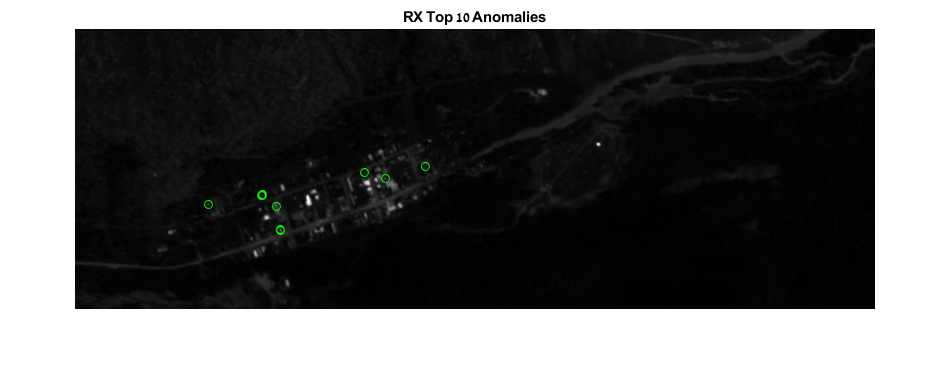
\includegraphics[width=\maxwidth{95.53437029603613em}]{figure_0}
\end{center}


\matlabheading{SSRX Algorithm}

\begin{par}
\begin{flushleft}
The SSRX algorithm adds a preprocessing step to the RX algrotihm - performing PCA and keeping only low variance PCs.
\end{flushleft}
\end{par}

\begin{par}
\begin{flushleft}
the formula for PCA is given by: 
\end{flushleft}
\end{par}

\begin{par}
$$X_{\mathrm{PCA}} =\left(X-m\right)\phi {\;}^{-1} V_q$$
\end{par}

\begin{par}
$$\begin{array}{l}\linebreak 
m-\textrm{the}\;\textrm{per}\;\textrm{channel}\;\textrm{mean}\;\textrm{of}\;X\\\linebreak 
\phi -\textrm{the}\;\textrm{covariance}\;\textrm{matrix}\\\linebreak 
V_q -a\;\textrm{matrix}\;\textrm{where}\;\textrm{every}\;\textrm{column}\;\textrm{is}\;\textrm{an}\;\textrm{eigen}\;\textrm{vector}\;\textrm{of}\;\phi \;\mathrm{while}\;\mathrm{ommiting}\;\mathrm{the}\;q\;\mathrm{eigen}\;\mathrm{vectors}\;\mathrm{that}\;\mathrm{correspond}\;\mathrm{to}\;\mathrm{the}\;\mathrm{highest}\;\mathrm{variance}\;\mathrm{eigen}\;\mathrm{values}\linebreak 
\end{array}$$
\end{par}

\begin{par}
\begin{flushleft}
Given $X_{\mathrm{PCA}}$ we can now run RX to obtain SSRX:
\end{flushleft}
\end{par}

\begin{par}
$$\mathrm{SS}\textrm{RX}={\left(\overrightarrow{X_{\mathrm{PCA}} } -\overrightarrow{m_{\mathrm{PCA}} } \right)}^T {\phi_{\mathrm{PCA}} }^{-1} \left(\overrightarrow{X_{\mathrm{PCA}} } -\overrightarrow{m_{\mathrm{PCA}} } \right)>\textrm{Threshold}$$
\end{par}

\begin{matlabcode}
q = 120;
[V, D] = eigs(phi,126);
V5 = V(:,6:end);    % deleting first 5 PC
V50 = V(:,51:end);  % deleting first 50 PC
V120 = V(:,121:end);% deleting first 120 PC
data_pca2D5 = reshape(X_MINUS_M,x_size*y_size,num_of_bands) * V5;
data_pca2D50 = reshape(X_MINUS_M,x_size*y_size,num_of_bands) * V50;
data_pca2D120 = reshape(X_MINUS_M,x_size*y_size,num_of_bands) * V120;

data_pca5   = hyperConvert3d(data_pca2D5', x_size,y_size,num_of_bands);
data_pca50  = hyperConvert3d(data_pca2D50', x_size,y_size,num_of_bands);
data_pca120 = hyperConvert3d(data_pca2D120', x_size,y_size,num_of_bands);

\end{matlabcode}

\begin{par}
\begin{flushleft}
Now that we have the preprocessed data, we can run the RX algorithm on it to get SSRX:
\end{flushleft}
\end{par}

\begin{matlabcode}
%calc phi_inv
[X_MINUS_M_PCA5,phi_pca5]=HSI_MF_params(data_pca5);
[X_MINUS_M_PCA50,phi_pca50]=HSI_MF_params(data_pca50);
[X_MINUS_M_PCA120,phi_pca120]=HSI_MF_params(data_pca120);

phi_pca_inv5 = pinv(phi_pca5);
phi_pca_inv50 = pinv(phi_pca50);
phi_pca_inv120 = pinv(phi_pca120);

%init empty results matrices
SSRX5   = zeros(x_size,y_size);
SSRX50  = zeros(x_size,y_size);
SSRX120 = zeros(x_size,y_size);

for x = 1:x_size
    for y = 1:y_size
        x_minus_m5 = squeeze(X_MINUS_M_PCA5(x,y,:));
        x_minus_m50 = squeeze(X_MINUS_M_PCA50(x,y,:));
        x_minus_m120 = squeeze(X_MINUS_M_PCA120(x,y,:));
        
        SSRX5(x,y) = x_minus_m5' * phi_pca_inv5 * x_minus_m5;
        SSRX50(x,y) = x_minus_m50' * phi_pca_inv50 * x_minus_m50;      
        SSRX120(x,y) = x_minus_m120' * phi_pca_inv120 * x_minus_m120;
    end
end
SSRX5= SSRX5';
SSRX50= SSRX50';
SSRX120= SSRX120';
SSRX5_filt = SSRX5 > mean(SSRX5(:)) + 3*std(SSRX5(:));
SSRX50_filt = SSRX50 > mean(SSRX50(:)) + 3*std(SSRX50(:));
SSRX120_filt = SSRX120 > mean(SSRX120(:)) + 3*std(SSRX120(:));
\end{matlabcode}

\vspace{1em}


\matlabheading{Top 10 Anomalies}

\begin{par}
\begin{flushleft}
Let's look at the top 10 results of the RX and the SSRX. Firstly, let's compare the different flavours of SSRX to see if there's any change in top anomalies:
\end{flushleft}
\end{par}

\begin{matlabcode}
[~, idxs_pca5] = maxk(SSRX5(:), 10);
[~, idxs_pca50] = maxk(SSRX50(:), 10);
[~, idxs_pca120] = maxk(SSRX120(:), 10);
[row_pca5,col_pca5] = ind2sub(size(SSRX5),idxs);
[row_pca50,col_pca50] = ind2sub(size(SSRX50),idxs);
[row_pca120,col_pca120] = ind2sub(size(SSRX120),idxs);
figure; imshow(data(:,:,1)',[]); hold on; 
plot(col_pca5,row_pca5,'or')
plot(col_pca50,row_pca50,'xg')
plot(col_pca50,row_pca50,'sb')
legend('Delete 5 PC', 'Delete 50 PC', 'Delete 120 PC')
title('SSRX Top 10 Anomalies')
\end{matlabcode}
\begin{center}
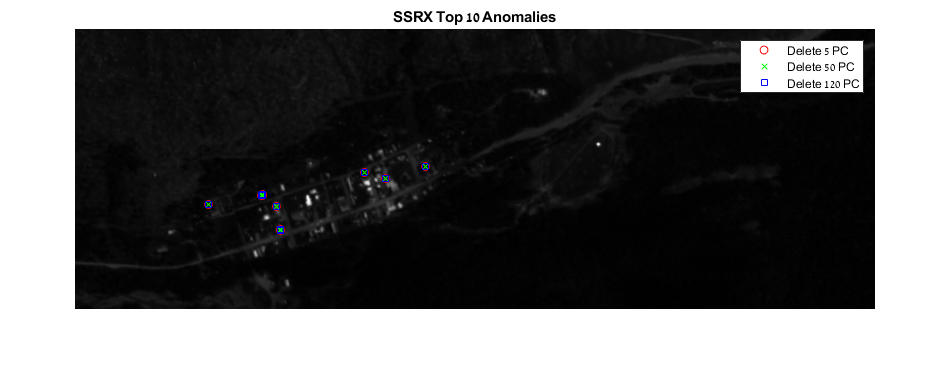
\includegraphics[width=\maxwidth{95.53437029603613em}]{figure_1}
\end{center}

\begin{par}
\begin{flushleft}
\textbf{Conclusion:} top 10 SSRX anomalies stay the same regardless of how many PCs we cut off.
\end{flushleft}
\end{par}

\vspace{1em}

\begin{par}
\begin{flushleft}
Now let's compare one the SSRX flavours to RX:
\end{flushleft}
\end{par}

\begin{matlabcode}
figure; imshow(data(:,:,1)',[]); hold on; 
plot(col,row,'xr')
plot(col_pca5,row_pca5,'og')
title('SSRX5 vs RX Top 10 Anomalies')
legend('RX','SSRX5')
\end{matlabcode}
\begin{center}
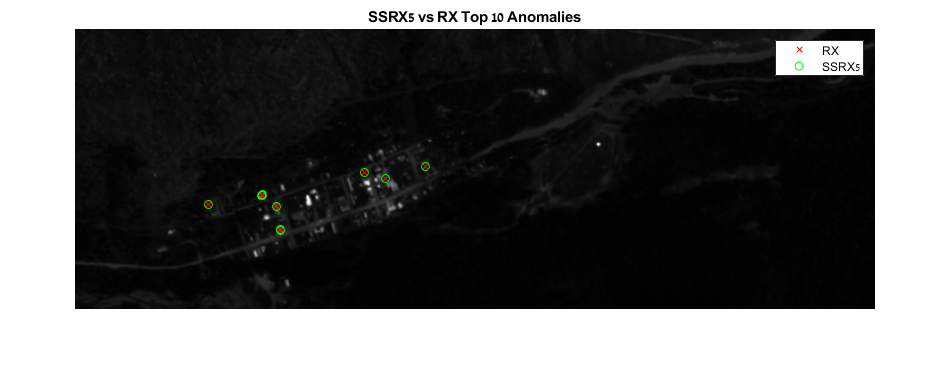
\includegraphics[width=\maxwidth{95.53437029603613em}]{figure_2}
\end{center}

\begin{par}
\begin{flushleft}
\textbf{Conclusion:} top 10 RX anomalies remain for SSRX as well.
\end{flushleft}
\end{par}


\matlabheading{Scatter Plot Comparison}

\begin{par}
\begin{flushleft}
Based on the results above, the difference between the 2 algorithms (if exists) is in the lower scored anomalies. Let's try to look at that:
\end{flushleft}
\end{par}

\begin{matlabcode}
h1=figure; 
spy(RX_filt,'or'); 
hold on;
spy(SSRX5_filt,'xg');
legend('RX','SSRX');
title('RX vs SSRX (deleting 5 highest variance PCs');
set(h1, 'Position', [0 0 1200 600])
\end{matlabcode}
\begin{center}
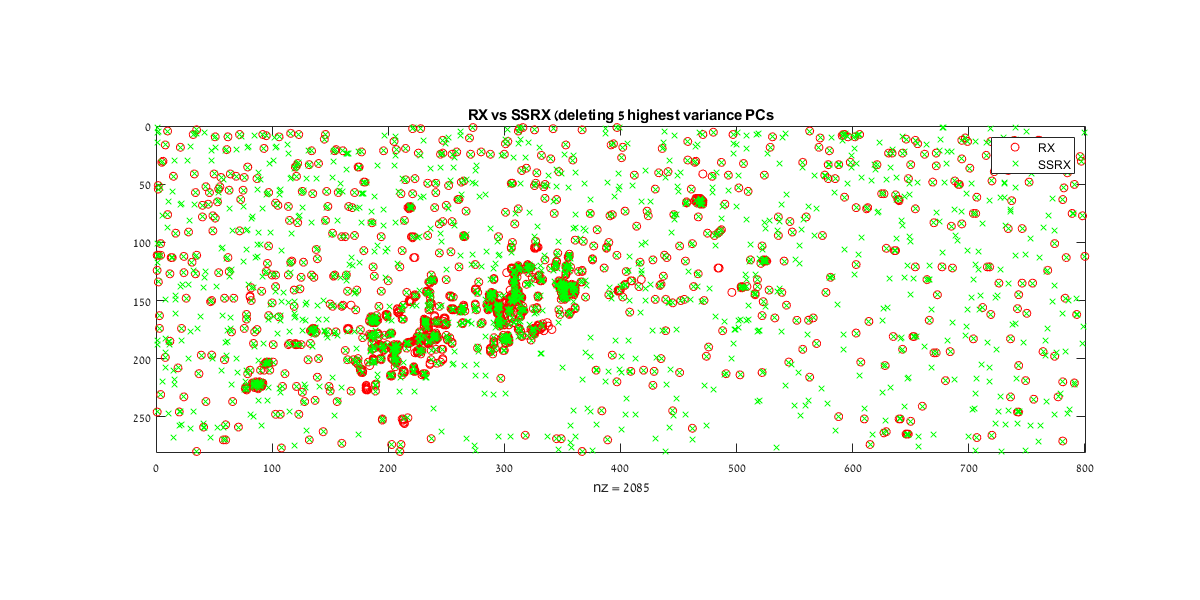
\includegraphics[width=\maxwidth{120.42147516307075em}]{figure_3}
\end{center}
\begin{matlabcode}

h2=figure; 
spy(RX_filt,'or'); 
hold on;
spy(SSRX50_filt,'xg');
legend('RX','SSRX50');
title('RX vs SSRX (deleting 50 highest variance PCs');
set(h2, 'Position', [0 0 1200 600])
\end{matlabcode}
\begin{center}
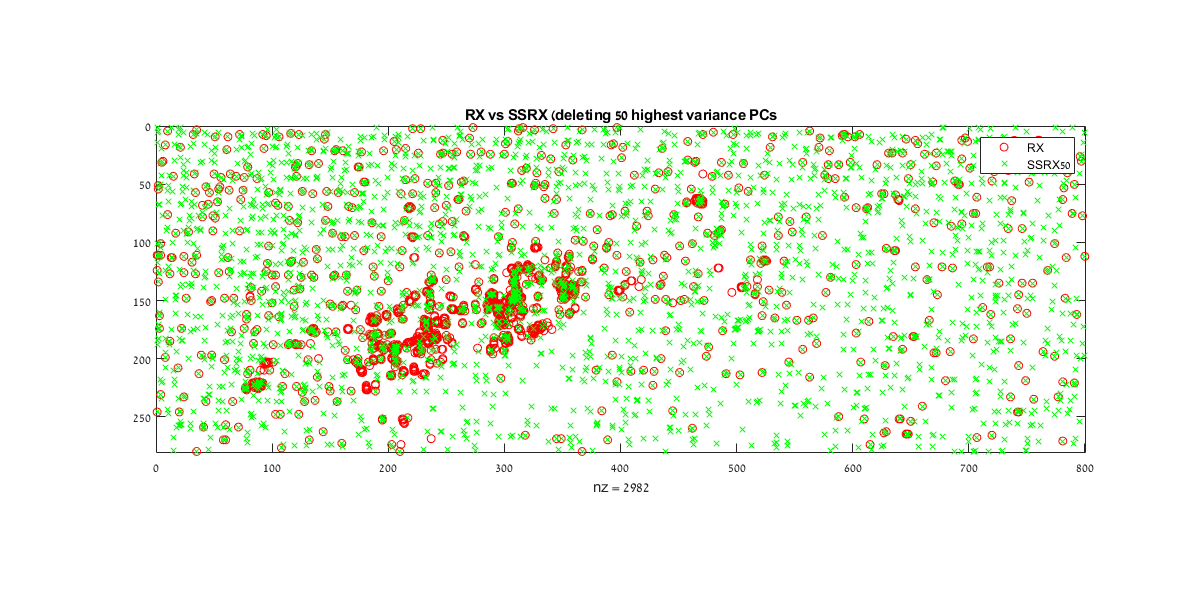
\includegraphics[width=\maxwidth{120.42147516307075em}]{figure_4}
\end{center}
\begin{matlabcode}

h2=figure; 
spy(RX_filt,'or'); 
hold on;
spy(SSRX120_filt,'xg');
legend('RX','SSRX120');
title('RX vs SSRX (deleting 120 highest variance PCs');
set(h2, 'Position', [0 0 1200 600])
\end{matlabcode}
\begin{center}
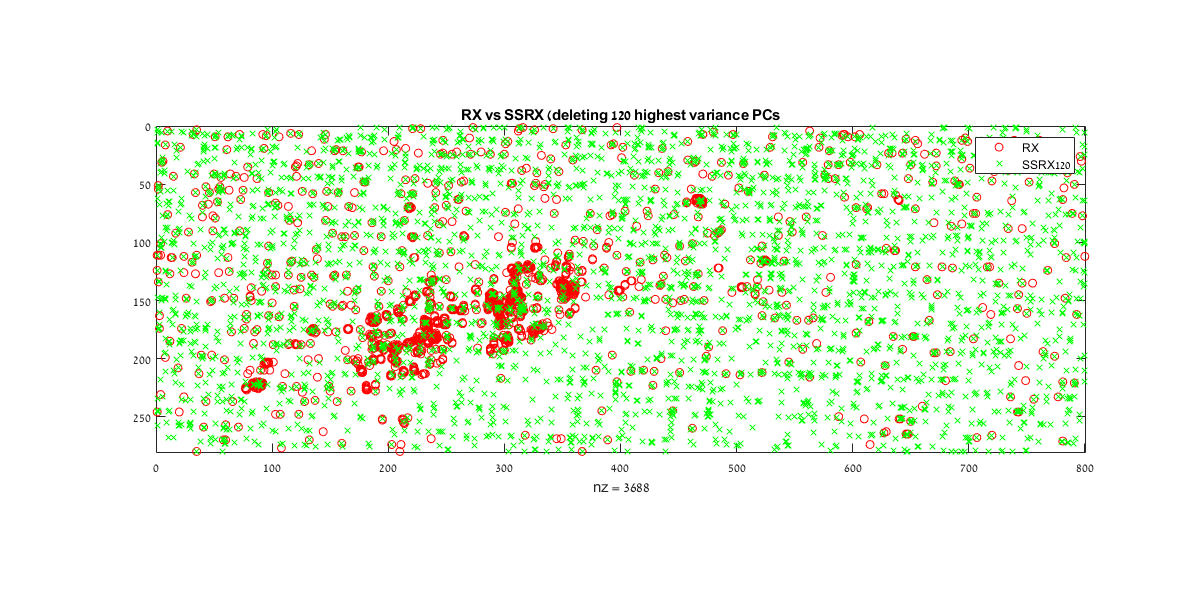
\includegraphics[width=\maxwidth{120.42147516307075em}]{figure_5}
\end{center}

\begin{par}
\begin{flushleft}
\textbf{Conclusion:} Seems like RX provides best results over all SSRX variants, and that the best SSRX variant is obtained by deleting only 5 hig variance PCs.
\end{flushleft}
\end{par}


\begin{par}
\begin{flushleft}
Histogram of all scores
\end{flushleft}
\end{par}

\begin{matlabcode}
[RX_val,RX_bins]=histcounts(RX,1000);
[SSRX5_val,SSRX5_bins]=histcounts(SSRX5,1000);
[SSRX50_val,SSRX50_bins]=histcounts(SSRX50,1000);
[SSRX120_val,SSRX120_bins]=histcounts(SSRX120,1000);
figure;
plot(RX_bins(1:1000),RX_val);
hold on;
plot(SSRX5_bins(1:1000),SSRX5_val);
plot(SSRX50_bins(1:1000),SSRX50_val);
plot(SSRX120_bins(1:1000),SSRX120_val);
xlim([-100 1000]);
legend('RX','SSRX5','SSRX50','SSRX120');
title('Histograms');
\end{matlabcode}
\begin{center}
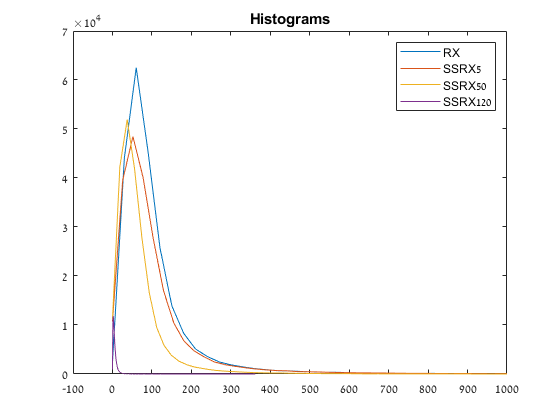
\includegraphics[width=\maxwidth{56.196688409433015em}]{figure_6}
\end{center}

\end{document}
